%Vorlesung vom 23.11.17

\begin{document}
\section{Family-wise Error Rate (FWER) }
\[ \text{FWER}_{\theta}(\phi)  := P \left( \bigcup_{j\in I_{0}(\theta)} \{ \phi_j = 1\} \right) \]
$\mathrel{\widehat{=}}$ Wahrscheinlichkeit für einen multiplen Fehler 1.Art (falls $\theta$ der wahre Parameter ist) \\
$\rightarrow \phi$ heißt \underline{Test zum multiplen Niveau $\alpha$ }, falls
\[ \text{FWER}_{\theta}(\phi) \leq \alpha \]
für alle $\theta \in \Theta $

\subsection{Bonferon}
\[ \phi = (\phi_{1},...,\phi{m})^T \text{  - multipler Test} \]
\[ P(\{\phi_j = 1\} \leq \underbrace{\frac{\alpha}{m}}_{\text{Bonferoni-Korrektur}} \text{ für alle } \theta \in H_0^{(j)}, j \in \{1,...,m\} \]
\[ \Rightarrow \text{FWER}_{\theta}(\phi) \leq \alpha \text{ für alle }\theta \in \Theta \]
$\rightarrow$ Ist jedes $\phi_j, j \in \{1,...,m\}$ ein Test zum Niveau $\tilde{\alpha} := \frac{\alpha}{m}$, so ist $\phi$ ein multipler Test zum Niveau $\alpha$

\subsection{\v Sid\'ak}
\begin{itemize}
 \item $ \phi = (\phi_{1},...,\phi{m})^T \text{  - multipler Test} $
 \item $\phi_j (X), j \in \{1,...,m \}$ unabhängig
\end{itemize}
\[ P(\{\phi_j = 1\} ) \leq 1-(1-\alpha)^{\frac{1}{m}} \text{ für alle } \theta in \Theta, j \in \{1,...,m\}\]
\[ \Rightarrow \text{FWER}_{\theta}(\phi) \leq \alpha \text{ für alle }\theta \in \Theta \]
$\rightarrow$ Ist jedes $\phi_j, j \in \{1,...,m\}$ ein Test zum Niveau $\tilde{\alpha} := 1-(1-\alpha)^{\frac{1}{m}}$ und sind alle Tests voneinander unabhängig so ist $\phi$ ein multipler Test zum multiplen Niveau $\alpha$ \\
Es gilt:
\[ \frac{a}{m} \leq 1-(1-\alpha)^{\frac{1}{m}} \]
$\rightarrow$\v Sid\'ak ist weniger konservativ als Bonferoni, wenn die Tests unabhängig voneinander sind \\

\subsection{p-Wert:}
Der p-Wert ist die Wahrscheinlichkeit dafür, dass unter der Nullhypothese die Prüfgröße T (statistischer Test) den Wert T(x) oder einen extremeren Wert annimmt, wobei $x-(x_1,...,x_n)^T$ die Realisierung der Stichprobe $X=(X_1,...,X_n)^T$ ist
\begin{center}
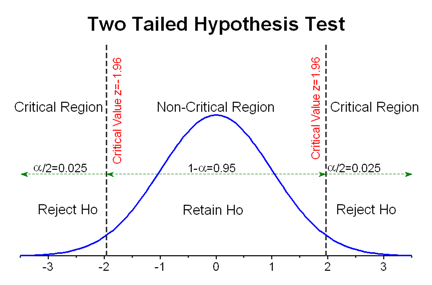
\includegraphics[scale=0.8]{twotailedtest.png}
\end{center}

\subsection{Bonferroni-Holm-Test}
\begin{itemize}
 \item $\phi=(\phi_1,...,\phi_m)^T $ - multipler Test
 \item $\phi=(p_1,...,p_m)^T $ - zu Tests gehörende p-Werte
 \item $p_{(1)} \leq ... \leq p_{(m)} $ - geordnete p-Werte
 \item $H_{(1)},...,H_{(m)} $ - zu geordneten p-Werten gehörende Nullhypothesen
 \item $\tilde{\alpha}_j := 
	\begin{cases}
	 \frac{a}{j} & , \text{ falls } p_j(X) \text{ nicht unabhängig } \\
	 1-(1-\alpha)^{\frac{1}{j}} & , \text{ falls } p_j(X) \text{ unabhängig }
	\end{cases}
	$
 \item $\phi^{BH}=(\phi_1^{BH},...,\phi_m^{BH})^T$ mit \\
 $\phi_j^{BH} := 
      \begin{cases}
       1 & ,\text{ falls } j \leq j^* \\
       0 & ,\text{ falls } j > j^* \\
      \end{cases}
      $\\
      wobei $j^* =\max\{ \max\{j \in I_0(\theta) : p_{(k)} \leq \tilde{\alpha}_{m-k+1}$ für alle $k \in \{1,...,j\}\}, 0 \}$
\end{itemize}
\paragraph{Beispiel}
\[ p_{(1)} \leq \frac{\alpha}{m} = \tilde{\alpha}_1 \]
\[ p_{(2)} \leq \frac{\alpha}{m-1} = \tilde{\alpha}_1 \]
\[ p_{(3)} \textcolor{red}{>} \frac{\alpha}{m-2} = \tilde{\alpha}_1 \]
\[ p_{(4)} > \frac{\alpha}{m-3} = \tilde{\alpha}_1 \]
\[ p_{(5)} \leq \frac{\alpha}{m-4} = \tilde{\alpha}_1 \]
$\Rightarrow \phi^{BH}$ ist multipler Test zum multiplen Niveau $\alpha$ 
\paragraph{Info:}
Bonferroni-Holm ist beser als Bonferroni bzw. \v Sid\'ak bzgl. Typ-II-Fehlern\\
$\rightarrow$ ''step-down''-Verfahren

\section{False Discover Rate (FDR) }
\begin{tabular}{c|c|c|c}
0-Hyp\ Test & nicht ablehnen & ablehnen & \\ \hline
wahr & \cellcolor{yellow!25} $m_0 (\theta) - V(\theta)$ & \cellcolor{yellow!25}$V(\theta)$ & \cellcolor{yellow!25}$m_0(\theta)$\\ \hline
falsch &\cellcolor{yellow!25}$m_A (\theta) - S(\theta)$  &\cellcolor{yellow!25} $S(\theta)$ &\cellcolor{yellow!25} $m_A(\theta)$\\ \hline
& \cellcolor{red!25}$m-R(\theta)$ & \cellcolor{red!25}$R(\theta)$ & m\\
\end{tabular}
\todo[inline]{yellow=unbekannt\\ red=bekannt}

\begin{itemize}
 \item $m$ - Anzahl der Tests \\
 \item $m_0 (\theta)$ - Anzahl der unter $\theta$ wahren Nullhypothesen \\
 \item $m_A (\theta)$ - Anzahl der unter $\theta$ falschen Nullhypothesen \\
 \item $R(\theta) = \sum\limits_{j=1}^m \phi_j$ - Anzahl unter $\theta$ verworfener Nullhypothesen
 \item $V(\theta) = \sum\limits_{j \in I_0(\theta)} \phi $ (zufällige) Anzahl unter $\theta$ fälschlicherweise verworfener Nullhypothese 
 \item $S(\theta) = \sum\limits_{j \in I_A(\theta)} \phi $ (zufällige) Anzahl unter $\theta$ korrekterweise verworfener Nullhypothese 
\end{itemize}

\[ \text{FDR}_{\theta}(\phi) := \text{E} \left( \frac{V(\theta}{\max\{R(\theta),1\}}\right) \]
$\rightarrow$ Multipler Test $\phi$ heißt \underline{FDR-kontrollierend zum Niveau $\alpha$}, falls
\[ \text{FDR}_{\theta}(\phi) \leq \alpha \text{ für alle } \theta \in \Theta \]

\end{document}